\documentclass[11pt]{article}
\usepackage{amsmath}
\usepackage{listings}
\usepackage{graphicx}


\begin{document}
\title{PHY 480 Project 1}
\author{Benjamin Brophy}
\maketitle

\section{Abstract}

In this project I will numerically solve the Poisson equation with Dirichlet boundary conditions by rewriting it as a set of linear equations. The Poisson equation is a second order differential equation, and here we discretize the equation into $N$ points and use an $h^2$ order approximation for the second derivative. The equation could be solved with standard LU decomposition with the order of $N^3$ operations, but here we implement the Thomas algorithm for systems with tridiagonal matrices to solve it on the order of $N$ flops. I further simplified the Thomas algorithm for the case that the off-diagonal elements of the tridiagonal matrix are all -1. The implementation of both methods show the Thomas Algorithm completes much faster, and produces a satisfactory solution to the Poisson equation.

\section{Introduction}
The Poisson equation describes the electrostatic potential $\Phi$ from a charge distribution $\rho(\mathbf{r})$. For three dimensions it is:
$$ \bigtriangledown^2\Phi = -4\pi \rho (\mathbf{r})$$

For the spherically symmetric case, both the distribution and potential only depend on r, so we can write a one dimensional form:
$$\frac{1}{r^2}\frac{d}{dr}\left(r^2\frac{d\Phi}{dr}\right)=-4\pi\rho(r)$$

Letting $\Phi(r) = \phi(r)/r$ we can rewrite this as 

$$\frac{d^2\phi}{dr^2}=-4\pi r\rho(r)$$

By function of $r$ on the right $f(r)=4\pi r\rho(r)$,  and letting $\phi \rightarrow u$ and $u \rightarrow x$, we obtain

$$-u''(x)=f(x)$$

In our case, we will take $f(x)=100e^{-10x}$ as our source function on $x\in[0,1]$ with $u(0)=u(1)=0$ as our boundary conditions.

\section{Methods}
We are solving the equation $-u''(x)=f(x)$ for $u(x)$, where $f(x)=100e^{-10x}$, on $x\in[0,1]$ with $u(0)=u(1)=0$. This is discretized to $N$ grid points $x_i=ih$ with spacing $h=\frac{1}{N+1}$. The discretized approximate of $u(x_i)$ is $v_i$. The $h^2$ order approximation of $f(x)$ is then $$\frac{-v_{i+1}+2v_i-v_{i+1}}{h^2}=f_i$$.
Let $b_i\in\mathbf{b}$ be defined as $b_i=h^2f_i$. Then
$$-v_{i+1}+2v_i-v_{i+1}=b_i$$
$$\begin{matrix}
(0& \cdots&0&-1& 2 & -1 & 0 & \cdots & 0)
\end{matrix}
\begin{matrix}
(v_0&\cdots&v_{i-1}&v_{i}&v_{i+1}&\cdots&v_n)
\end{matrix}^T=b_i$$

$$\begin{bmatrix}
2&-1&0&\cdots&\cdots&0\\
-1&2&-1&0&\cdots&\cdots\\
0&-1&2&-1&0&\cdots\\
\cdots&\cdots&\cdots&\cdots&\cdots&\cdots\\
\cdots&\cdots&\cdots&-1&2&-1\\
0&\cdots&\cdots&0&-1&2
\end{bmatrix}
\begin{bmatrix}
v_1\\\cdots\\v_i\\\cdots\\v_N
\end{bmatrix}
=
\begin{bmatrix}
b_1\\\cdots\\b_i\\\cdots\\b_N
\end{bmatrix}$$
Thus,
$$
\mathbf{Av}=\mathbf{b}
$$

To solve this matrix I will use a simplified version of Gaussian elimination for tridiagonal matrices called the Thomas algorithm, further simplified for the values of this tridiagonal matrix. The first step is forward substitution. After this step, all elements other than the diagonal and elements 1 to the right are 0, all values 1 right of the diagonal are -1, so we only need to compute the new diagonal values, $\tilde{d}_i$, and new values of the right hand side, $\tilde{b}_i$. ($\tilde{d}_1=d_1=2$, $\tilde{b}_1=b_1$)
$$\tilde{b_i} = b_i - \frac{a_ic_{i-1}}{\tilde{b}_{i-1}}$$
$$\tilde{d_i} = d_i - \frac{a_{i-1}\tilde{d}_{i-1}}{\tilde{b}_{i-1}}$$
Then I completed backwards substitution to solve for $v_i$ with the following algorithms ($v_N=\tilde{b}_N$):
$$x_i=\frac{\tilde{d}_i-c_ix_{i+1}}{\tilde{b}_i}$$


General Gaussian Elimination or LU factorization solutions would take about $\frac{2}{3}N^3$ flops to solve the equation. The Thomas algorithm would in general require about $4N$ flops for each forwards and backwards substitution for a total of $8N$ flops, but the simplified algorithm for this matrix reduces that to $2N$ flops for each forwards and backwards substitution, for a total of about $4N$ flops.

\section{Analysis}

The resulting solutions for $N=10,100,1000,10000$ are plotted along with the analytical solution $u(x)=1-(1-exp(-10))x-exp(-10x)$ on the following page. The code used is at the end of the report. The solution is a rough but somewhat looking approximation at N=10, and as far as can be seen here, looks like a near perfect representation of the f(x) as n takes on values of 1000 and higher.

\begin{figure}
	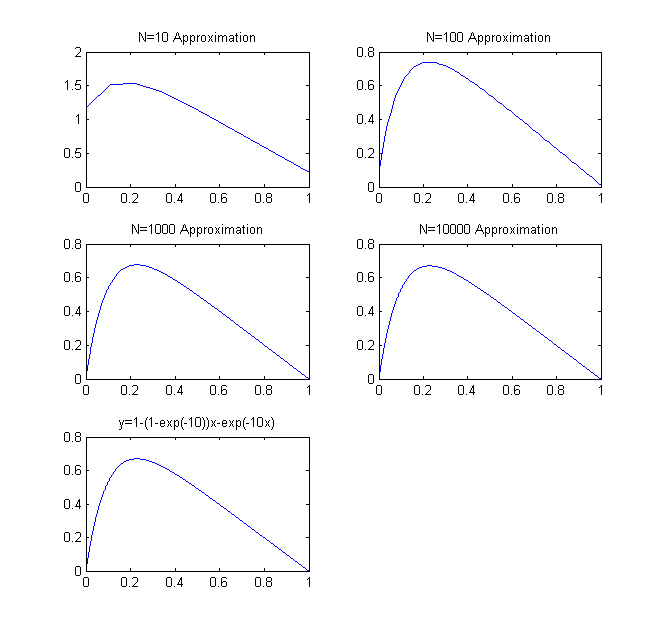
\includegraphics[width=\linewidth]{variousNplots}
	\caption{The solution is a rough but somewhat looking approximation at N=10, and as far as can be seen here, looks like a near perfect representation of the f(x) as n takes on values of 1000 and higher.}
\end{figure}

For each value of N, for each step i the log of the relative error was measured with regard to the actual value $u_i=u(x_i)$, where $u(x)$ is the analytical solution $u(x)=1-(1-exp(-10))x-exp(-10x)$.
$$\epsilon_i=log_{10}\bigg(\bigg|\frac{[v_i-u_i]}{u_i}\bigg|\bigg)$$
Here are is the maximum error at any point $x_i$ for each $N$. The error seems to decrease about as the increase in the order of magnitude of N.

$$
\begin{array}{|c|c|}
\mathbf{N} & \mathbf{Max Error}\\
\hline
10 & 0.301744\\
100 & 0.0374884\\
1000 & 0.00384884\\
10000 & 0.000385926
\end{array}
$$

When measuring the time for various my solver using "time.h" in C++, even for $N=10^5$, the solution did not take long enough to register on a scale of seconds. My solver performs on the order of $N$ flops. However, LU decomposition takes on the order of $N^3$ flops. Here are the results of my measurement of solving using LU decomposition.

$$
\begin{array}{|c|c|}
\mathbf{N} & \mathbf{Time (s)}\\
\hline
10 & 0\\
100 & 0\\
1000 & 2\\
10000 & 5194\\
100000 & N/A
\end{array}
$$

So, it took about 1.44 hours to solve the problem with $N=10^4$. When I attempted to solve the $N=10^5$ matrix using LU decomposition, it never finished in hours, which makes sense since it should take on the order of $10^3$ longer than the solution of the $N=10^4$ case.

\section{Conclusions}
We were able to numerically solve the Poisson equation for the source function  $f(x)=100e^{-10x}$. The Thomas algorithm was successful in creating an accurate numerical model, and in Figure 1 we can see the numerical model approximates the analytical solution very nicely. As N increases, the error of the approximation decreases on the order of N. We also showed that the implementation of the Thomas Algorithm solved the equation much quicker than LU decomposition as N grew very large, as was expected. Solving the problem increased over 1000 times longer as the number of point increased by 10 times in the LU decomposition, while the Thomas Algorithm took less than a second to solve for at least 100000 points.

\section{Bibliography}
\begin{thebibliography}{widestlabel}
	\bibitem{morten}
	Hjorth-Jensen, M. (n.d.). Computational Physics Lectures: Linear Algebra methods. Retrieved from http://compphysics.github.io/ComputationalPhysicsMSU/doc/pub/linalg/pdf/linalg-minted.pdf
\end{thebibliography}



\section{Code}
Here is the code used in this project, in C++:

\begin{lstlisting}
using namespace std;

#include <iostream>
#include <cmath>
#include <fstream>
#include <string>
#include "time.h"
#include "../../ComputationalPhysicsMSU/doc/Programs/LecturePrograms/programs/cppLibrary/lib.h"

int main()
{
clock_t start_alg, finish_alg;
cout << "N?" << endl; //size of matrix
int N, i, j;
double h;
cin >> N;
double n = N;
h = 1/(n+1);
double *A = new double[N];
// initialize A array, representing diagonal of A, all elements = 2
for(i=0 ; i < N ; i++) {
A[i] = 2.0;}

double *B = new double[N];
// initialize B = h^2*f(x) = 100*exp(-10x)
for(i=0 ; i < N ; i++) {
B[i]=h*h*100*exp(-10*h*i);
}

start_alg=clock();
// forward substitution
for(i=1 ; i < N ; i++) {
A[i]=A[i]-(1/A[i-1]);
B[i]=B[i]+B[i-1]/A[i-1];
}

// backward substitution
double *X = new double[N];;
X[N-1] = B[N-1]/A[N-1];
for(i=1 ; i < N ; i++) {
X[N-1-i]=(B[N-1-i]+X[N-i])/A[N-1-i];
}
finish_alg=clock();

double *E = new double[N];
double u, x;
double maxerror = 0.0;

//Finding error at each point, and maximum error
for(i=1 ; i < N ; i++) {
x = i*h;
u = 1 - (1 - exp(-10))*x - exp(-10*x);
E[i]= log10(abs((X[i]-u)/u));
if (E[i]>maxerror){maxerror = E[i];}
}

cout << "Max Error: " << maxerror << endl;

//write results to output file
std::string N_str = std::to_string(N);
std::string filename = "N" + N_str + ".txt";
ofstream myfile (filename);
if (myfile.is_open())
{
for(int count = 0; count < N; count ++){
myfile << X[count] << "\n" ;
}
myfile.close();
}

cout << "Time Alg: " << ((finish_alg-start_alg)/CLOCKS_PER_SEC)<<endl;

delete [] A; delete [] B; delete [] X; delete [] E;

int *indx;
indx = new int[N];
double d;
double **Z;
Z=new double*[N];
for ( i = 0; i < N; i++){
Z[i] = new double[N];
}
for ( i = 0; i < N; i++){
for ( j = 0; j < N; j++){
if (i==j){
Z[i][j]=2.0;
}
else if (i==j+1 || j == i+1){
Z[i][j]=-1.0;
}
else{
Z[i][j]=0.0;
}

}
}
double *b = new double[N];
// initialize b = h^2*f(x) = 100*exp(-10x)
for(i=0 ; i < N ; i++) {
b[i]=h*h*100*exp(-10*h*i);
}

clock_t start_LU, finish_LU;
start_LU = clock();
// LU decompose the matrix
ludcmp(Z,N,indx,&d);
// Then backward substitution
lubksb(Z, N, indx, b);
finish_LU = clock();

cout << "Time LU: " << ((finish_LU-start_LU)/CLOCKS_PER_SEC)<<endl;

// Free space
delete [] b;
for ( i = 0 ; i < N; i++) delete [] Z[i];
delete [] Z;

return 0;
}

\end{lstlisting}

\end{document}